%% Los cap'itulos inician con \chapter{T'itulo}, estos aparecen numerados y
%% se incluyen en el 'indice general.
%%
%% Recuerda que aqu'i ya puedes escribir acentos como: 'a, 'e, 'i, etc.
%% La letra n con tilde es: 'n.
\chapter{Corazón y sus características}

El corazón es uno de los órganos mas importantes del cuerpo humano ya que es el encargado de bombear sangre a través de las venas por todo el cuerpo, tiene como dimensiones, 12 centímetros de largo, 9 centímetros de ancho y 6 centímetros de espesor, su peso ronda entre los 200 y 425 gramos.\newline

\begin{floatingfigure}[r]{3cm}

\includegraphics{imag/corazon.PNG}
%\captionof{Figura}{Un poliedro}
\end{floatingfigure}

Como tal esta formado por dos bombas que se les menciona como corazón derecho e izquierda el primero bombea sangre hacia los pulmones y el izquierdo bombea sangre por la circulación sistémica que lo lleva hacia los demás órganos del cuerpo.\newline
Se encuentra ubicado en la región del mediastino medio, justo entre los pulmones y la parte media del pecho, detrás del esternón, se apoya sobre el diafragma.\newline\newline
Como tal el corazón esta dividido en dos mitades incomunicadas entre si(Figura\ref{cavi}), una derecha y una izquierda, estas mitades se subdividen en dos cavidades conformando un total de 4 cavidades, la capa superior se llama aurícula y la cavidad inferior se llama ventrículo.\newline

En la figura \ref{cavi} observamos los principales componentes de las cavidades del corazón, estas son las partes mas importantes para obtener las señales correspondientes, esto ya que el corazón no tiene un movimiento  uniforme, si no que cada componente forma un patrón consecutivo en el cual su señal es independiente pero es consecuencia de un antecesor.

\begin{figure}[H]
   	\centering
		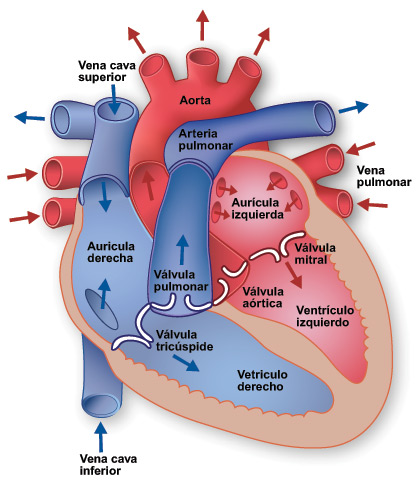
\includegraphics[width=6cm]{imag/cavidad.jpg}
		\caption{Cavidades.}
		\label{cavi}
\end{figure}


Como tal para que el corazón se contraiga es necesario que sus células musculares reciban un estímulo eléctrico. Este se genera en células especializadas (células marca pasos) del sistema de conducción, que originan el impulso por sufrir des polarizaciones espontáneas (automatismo).\newline

Cada cara del corazón la exploran unas derivaciones particulares: inferior(II, III, aVF), lateral alta (I, aVL), lateral baja (V5,v6), anterior(V3, V4), septo (V1, V2), posterior(V7,V8,V9), ventrículo derecho (V3R, V4R).
\chapter{Componentes electrónicos}
Dentro de los componentes mas importantes se encuentran los siguientes:\newline

\textit{Electrodos}: estos elementos son los encargados de recibir la señal proveniente del cuerpo humano (Figura 4.1), se adhiere a la piel y se agrega un desinfectante para evitar ruido para la señal.\newline
\begin{floatingfigure}[r]{4.5cm}
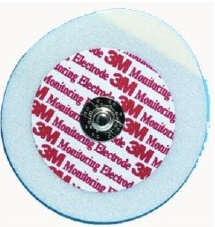
\includegraphics{imag/electrodo.PNG}
%\captionof{Figura}{Un poliedro}
\caption{Electrodos.}
		\label{electrodos}
\end{floatingfigure}

\textit{Cables para electrocardiógrafo}, estos son los medios de transmisión a través de los cuales es envía la información (señales eléctricas del corazón) y que tienen un aislante para no recibir perturbaciones externas.\newline

Esto permite que la señal entrante no tenga dentro de si demasiado ruido y se permita un correcto análisis de esta. El acondicionamiento de la señal se debe en mucho a la correcta colocación de este elemento.\newline

\begin{floatingfigure}[r]{1.0cm}
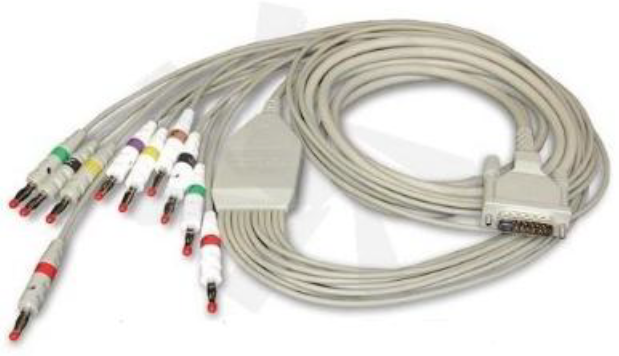
\includegraphics{imag/cables.PNG}
%\captionof{figure}{Un poliedro}
\end{floatingfigure}

\textit{Adaptadores}: Estos por su parte permiten que la señal que viene a través del medio de transmisión se incorpore al sistema para que el sistema interno ya trabaje con esta señal.\newpage
\begin{figure}[H]
   	\centering
		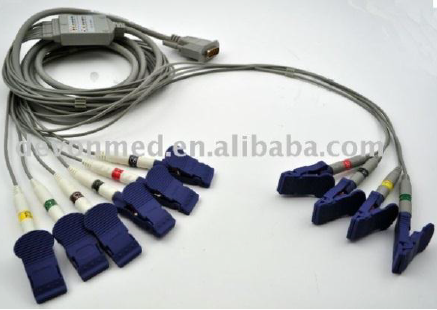
\includegraphics[width=6cm]{imag/adaptadores.PNG}
		\caption{Adaptadores.}
		\label{Adaptador}
\end{figure}
Por último tenemos el \textit{Smartphone}, este dispositivo puede ser de,cualquier modelo,gama y/o versión de Android. Esto debido a que se puede dar soporte a múltiples versiones de Android para que no tenga ningún problema de compatibilidad.\newline

Actualmente estos dispositivos ya poseen ciertas características de hardware como un procesador y memoria ram de buenas capacidades, por ello es que se adquiere la posibilidad de mostrar señales de electrocardiógrafo sin mayor problema, ya que otras aplicaciones para Android son mas demandantes y operan sin mayor problema.
\begin{figure}[H]
   	\centering
		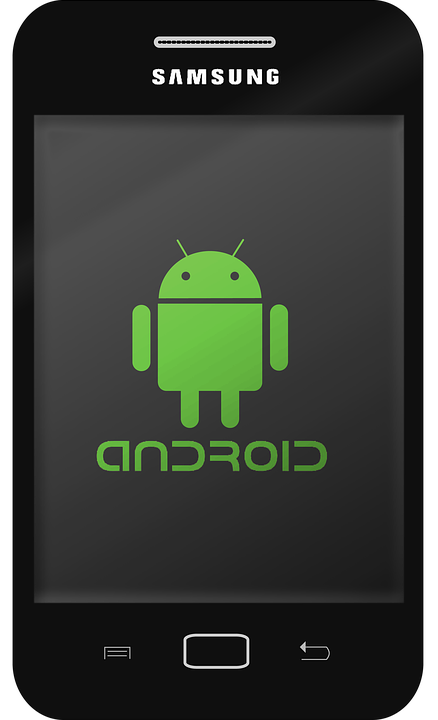
\includegraphics[width=3cm]{imag/smartphone.PNG}
		\caption{Smartphone.}
		\label{phone}
\end{figure}
\chapter{Sistema operativo Android}

El sistema operativo Android ó Android abreviandolo es un sistema de código abierto cuyo fin es desarrollar aplicaciones para teléfonos celulares y tabletas para el alcance de cualquier persona, es al igual que Linux, Ubuntu y otros sistemas un entorno que permite el desarrollo de nuevas herramientas sin fines de lucro, permite a los desarrolladores trabajar con entornos diseñados para la promoción del conocimiento.
\begin{floatingfigure}[r]{1cm}

\includegraphics{imag/mini.jpg}
%\captionof{figure}{Un poliedro}
\end{floatingfigure}
Para desarrollar una aplicación para Android se tienen distintas herramientas como lo son IDE´S (Entorno de Desarrollo Integrado) que facilitan la tarea de enlaces entre distintos lenguajes como lo son XML y java con las distintas clases que contiene dentro de si, esto da mayor empuje a las operaciones que se realizan dentro de las aplicaciones, sumado a esto tenemos que elegir una API (Interfaz de programación de aplicaciones).\newline

Una API dicho de manera cotidiana es la versión de Android que se posee en un dispositivo, está contiene distintas herramientas (o métodos) que se mejoran de una version a otra, corresponden a cada actualización del sistema y se les asigna un número.\newline
\begin{figure}
   	\centering
		
\includegraphics[width=4cm]{imag/androidmini.PNG}
		\caption{Android.}
		\label{andro}
\end{figure}
\newpage

Vamos a utilizar la API 21 para poder abarcar la mayor parte de dispositivos dentro de toda la gama de posibilidades. En particular para este proyecto utilizaremos Android Studio para desarrollar nuestra interfaz de usuario para visualizar las gráficas que se originen de nuestro circuito anterior.
